\subsection{Analog-to-Digital Converter} \label{sec:ADC_teori}
Outputtet fra målingerne er et analogt signal, der er kontinuert i tid og amplitude. 
For at kunne behandle signalet digitalt, skal dette konverteres fra analogt til digitalt. Denne konvertering sker ved anvendelse af en Analog-to-Digital Converter (ADC). 
Det analoge signal samples og kvantificeres under konverteringen, hvilket gør signalet diskret i tid og amplitude \citep{webster1998, morre2003}. 
Dette er illusteret på \autoref{fig:ADC_kon}. 

\begin{figure}[H]
\centering
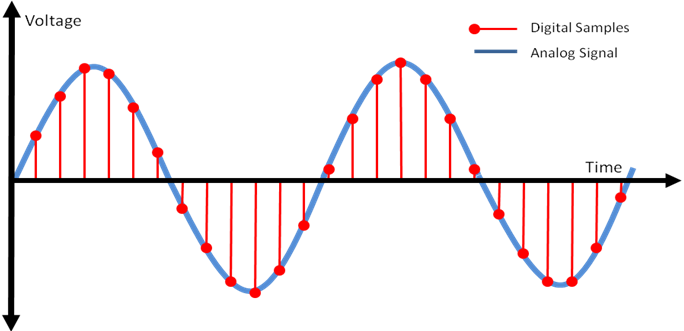
\includegraphics[width=0.7\textwidth]{figures/problemloesning/adc}
\caption{Illustration af konvertering fra analogt til digitalt signal. Den blå graf repræsenterer et analogt signal over tid. Den røde graf viser det konverterede signal, som er diskret i tid og amplitude.}
\label{fig:ADC_kon}
\end{figure}

\noindent
Samplingsprocessen sker ved diskretisering i tidsdomænet, hvor det kontinuerte signal konverteres til et diskret signal. 
Det er vigtigt at vælge en passende samplingsfrekvens for at undgå, at information fra det oprindelige signal ikke repræsenteres korrekt \citep{morre2003}. 
Ved for høj samplingsfrekvens vil en overføldig mængde data opsamles og derved benytte mere hukommelse samt gøre processering mere omstændig \citep{wolf2004}. 
En for lav samplingsfrekvens vil derimod give en fejltolkning af signalet, således kurven ikke kan repræsentere det oprindelige signal. Dette fremgår som alias \citep{morre2003}. 
Der accepteres en maksimal afvigelse på $2~\%$ for samplingfrekvensen, da det ikke ses af større betydning for samplingsfrekvensen. 
Dette gøres for så vidt muligt at tage højde for kvantificeringsfejl. 
For udvikling af dette system benyttes elektroder til opsamling af EMG samt to accelerometre, hvorfor det kræves, at ADC'en kan sample minimum tre inputs.
Ifølge Nyquists sætning er det hensigtsmæssigt, at samplingsfrekvensen er mindst det dobbelte af frekvensen i det oprindelige signal \citep{morre2003}. 
I praksis anbefales det at sample med det tidobbelte.

Kvantificering sker ved diskretisering af amplituden. 
Det oprindelige signals amplitudeværdier inddeles ved kvantificering i trin. 
Værdierne mellem to trin repræsenteres af én digital værdi, hvilket resulterer i, at forskellige analoge værdier kan konverteres til samme digitale værdi \citep{morre2003}. 
Amplitudeniveauer, der er tilgængelige til at repræsentere det analoge signal, determineres af antal bits. 
Ved en højere bitværdi vil det analoge signal repræsenteres bedre, hvilket er illustreret på \autoref{fig:ADC_bit}.

\begin{figure}[H]
\centering
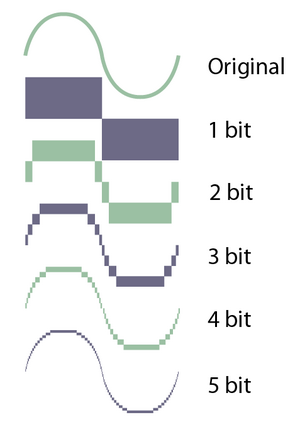
\includegraphics[width=0.6\textwidth]{figures/problemloesning/ADC_bit}
\caption{Illustration af betydningen af bits i forhold til et sinussignal. Ved en større bitværdi vil signalet repræsenteres tydeligere \citep{adc2010}.}
\label{fig:ADC_bit}
\end{figure}

\noindent
ADC'ens opløsning afhænger dens bitværdi. En ADC med en opløsning på 12-bit inddeles derfor i ${2}^{12}$ niveauer, hvilket svarer til 4096 niveauer. 
Dette giver en repræsentation af værdier fra 0 til 4096 eller fra -2048 til 2047. 
Sensitiviteten som ADC'en kan opnå, betegnes Least Significant Bit (LSB) og bestemmes ud fra \autoref{equ:LSB}, hvor Full Scale voltage Range (FSR) er det totale spændingsområde for ADC'en angivet i $V$, og $n$ er antallet af bits i ADC'en \citep{webster1998, wolf2004}.

\begin{equation} \label{equ:LSB}
LSB=\dfrac{FSR}{2^{n}}
\end{equation}

% = \dfrac{\dfrac{FSR}{{2}^{12}}}
\noindent
Hvis spændingen, der pålægges ADC'en overstiger dens arbejdsområde, vil dette resultere i, at signalet går i mætning \citep{webster1998, wolf2004}. 


\vspace{3mm}
\textbf{Krav:}
\begin{itemize}
\item Skal have en samplingsfrekvens 10 gange større end den højeste signalfrekvens
\begin{itemize}
\item Samplingsfrekvensen skal have en maksimal afvigelse på $2~\%$
\end{itemize}
%\item Skal have en samplingsfrekvens på $100~Hz$
\item Skal sample minimum tre inputs 
%\item Skal have en hastighed som ikke overskrider ADC'ens arbejdsområde \fxnote{Hvad vil hastigheden sige?}
\item Skal have en opløsning, der ikke forringer signalet
\item Skal undgå, at signalet ikke overstiger ADC'ens arbejdsområde

%\item Skal have en opløsning på minimum 10 bit
%\item Skal modtage en spændingsforsyning på $XX~V$

\end{itemize}

